%
\chapter{Implementation}\label{cha:Implementation}
%
In this chapter, the implementation part of this master's thesis will be described. The test track, which was implemented before by another student; the hardware part of the model automobile, which was used in this master's thesis; and finally, the software part which was programmed for detecting the lanes will all be  explained in detail.

In the Software section in \ref{sec:Software}, all methods programmed and utilized during this master's thesis will be descriebed. In order to better demonstrate the process, pictures of each step, as well as block diagrams of each method, will be shown.

%
\section{Test Track}\label{sec:Test Track}

As previously mentioned, the medium-term goal of this master thesis is attending the Carola-Cup at Braunschweig University, so the test truck was prepared according to the Carola-Cup criteria by Nicolas Acero Sepulveda, who also did his bachelor's thesis with this model automobile. For this test truck, two black PVC floor carpets were used and on these floor carpets, the lanes of the track were made by using white electrical tape. The straight part of the track was made on one of these PVC floor carpets and the curved part of track was made on the second PVC floor carpet. The straight part of the track is approximately 2 meters long and the curve radius of the curved part of test track is approximately 1 meter. This curve is the tightest curve at Carola-Cup, so with this, the test track can be tested in the worst case scenario. In the Carola-Cup competition, the track is much larger; however, for the purposes of this master thesis, a larger test track in not needed. \emph{\color{blue}In Figure \ref{fig:Test_Track}, the test track used in the testing of this master's thesis is shown.}


\begin{figure}[H]
	\centering
		\includegraphics[width=1\textwidth]{./Bilder/Test_Track.jpg}
	\caption{Test Track}
	\label{fig:Test_Track}
\end{figure}



%
\section{Hardware}\label{sec:Hardware}



%
\subsection{Model Auto}\label{sec:Model Auto}


During the course of this master's thesis, a model automobile was being used which was prepared for the Projectseminar 
Echtzeitsysteme at Technical University of Darmstadt. The chassis, steering mechanism, power train, and engine control 
were derived from the model-building of a Japanese company, Tamiya. The maximum velocity of the model automobile is 
approximately 1 m/s and the minimum steering radius is around 90 cm. 

\begin{figure}[H]
	\centering
	\hspace*{0cm}   
	\includegraphics[width=150mm,scale=1]{./Bilder/Model Auto.jpg}
	\caption{Model Auto}
\end{figure}

%
\subsection{Microcontroller and Main Board}\label{sec:Microcontroller and Main Board}


In this model automobile, there is a microcontroller and a main board. The microcontroller is used for controlling steering 
and receiving the measurements from ultrasonic sensors and hall effect sensors. The 16-bit microcontroller is from 
MB96300 series from Fujitsu company.

The main board on the model car is from PD10BI-MT ThinMini-ITX series from MiTAC company. This main board communicates 
with the microcontroller over via UART interface through USB connection. On this main board, there is an Intel 
Quadcore-Processor and an Intel HD Graphics card. Furthermore, there is an 8 GB DDR3-1600 RAM and 1Gbit/s Ethernet, VGA, HDMI, USB 2.0/3.0, SATA ports and an Intel Dual Band Wireless AC 7260 Network adapter, which is connected to two external WLAN antennas. A 60 GB Kingston SSD-Harddisk is connected over an integrated PCI-Express Port. A 3200 mAh Li-Fe battery is used as a power supply.
%

\subsection{Camera}\label{sec:Camera}


The camera is one of the main components of lane detection and accordingly, autonomous driving. For this thesis, I had 
to research the most suitable camera because all cameras have different properties.

At the beginning of the Projectseminar Echtzeitsysteme, the Logitech C270 HD Webcam was being used. The resolution of 
the camera is 1280x960 pixels and the Frame per Second (FPS) value is 30 Hertz (Hz) at a 640x480 pixel resolution. 
The field of View (FOV) is just 60 degrees. The problem with this camera is that if there is a curve, the camera 
cannot see all of the lanes, and thus is not very suitable for lane detection. When I started my master's thesis, there 
was a Kinect v2 camera on the model car.  The Kinect v2 camera was developed by Microsoft and released in 2013. This 
camera has a depth sensor with a resolution of 512x424 pixels and its FOV is 70x60 degrees. The FPS value is 30 Hz at 
a 512x424 pixel resolution. This camera also has a color camera with resolution of 1920x1080 pixels and a FOV of 
84.1x53.8 degrees. The FPS value is 30 Hz at a 1920x1080 pixel resolution. This camera had two main disadvantages for 
this master's thesis. The first disadvantage is the FOV value of camera. This value is better than the value of Logitech 
C270 camera but it is still not enough for curve lane detection. The second main disadvantage is the location of the 
color camera. The color camera of this camera is not in the middle of camera, but rather, on the right. This is a 
disadvantage for us because when there are curves going left as opposed to right, the camera is unable to see the 
left and even perhaps the middle lane of the truck. Thus, this is problematic for lane detection.

Due to these reasons, I had to choose a camera which has a sufficiently high FOV value. After doing research, I decided 
that the Genius Widecam F100 camera is the best choice for this master's thesis because this camera has a FOV value of 
120 degrees and it can also be used with the Linux Operating System. The resolution of this camera is 1920x1080 pixels 
and the FOV value is 120 degrees. The FPS is 30 Hz at a 1920x1080 pixel resolution. With this camera, it is possible 
to detect most if not all lanes, including when there are curves. 

\begin{figure}[H]
	\centering
	\hspace*{0cm}   
	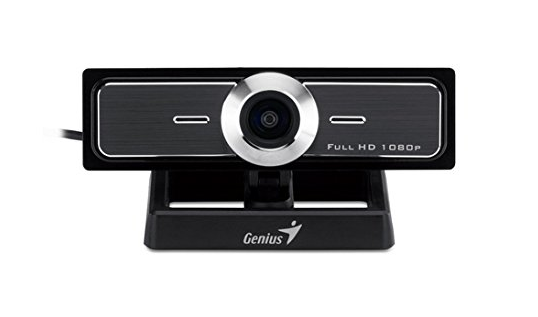
\includegraphics[width=150mm,scale=1]{./Bilder/Genius_F100_camera.png}
	\caption{Genius 120-degree Ultra Wide Angle Full HD Conference Webcam(WideCam F100) }
\end{figure}









\section{Response Time of the System}\label{sec:Response Time of the System}

Before the lane detection project was started, it was necessary to conduct an experiment with the system. The aim of this experiment was to measure the response time of the entire system. In order to measure it, the camera had to detect something and then the software had to set an I/O pin on the main board. The amount of time this process took was in fact the response time being searched for.

For this experiment, a camera, a power supply, an LED, and an oscilloscope were needed. A circuit with a power supply and an LED were designed. The LED was placed in a small box with a camera, and one probe of an oscilloscope was connected to the LED while its other probe was connected to an I/O Pin on the mainboard, which could be set with software.

Before the results were measured, the frequency of the camera was set to 10 Frames per Second(FPS) and the power supply was set to 3.28 Hz. square wave. This means that the LED is supposed to blink approximately every 305 ms.

After the supply was turned off, the LED started to blink. For this experiment, a small firmware able to detect the color red was written in order to detect when the red LED lit up.

The LED and a camera were placed together in a box and the box was closed, and so the inside of the box was totally dark. When the red LED lit up, the camera detected it and the firmware set an I/O pin on the main board. For this experiment, two different cameras were used and the results were very similar.


\begin{figure}[H]
 \centering
  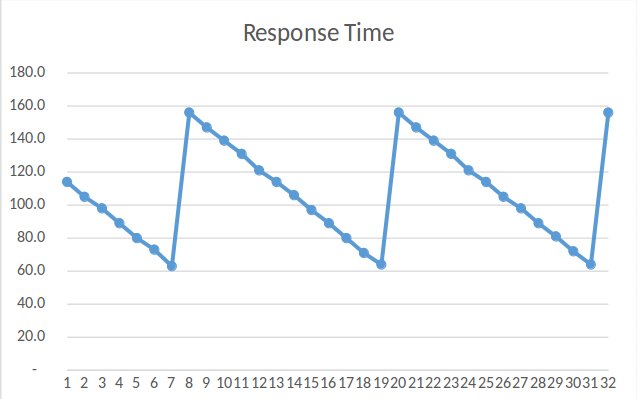
\includegraphics[width=0.8\textwidth]{./Bilder/Response_Time2.png}		 \caption{Response Time of the System}
  \label{fig:Response_Time_of_the_System}
\end{figure}


As in Figure \ref{sec:Response Time of the System} seen, the maximum response time of the system was 156 ms., the minimum
response time of the system was 63 ms., and the average time was 106.6 ms.




%
\section{Software}\label{sec:Software}


In this chapter, the software algorithms defined in this master's thesis will be focused on. With the aid of program flow charts and explanations of all their steps, the algorithms will themselves be better explained. In order to find the best solution, five different source code versions were generated. For all these source codes, the computing times were calculated and compared in terms of which solution can detect the lanes better. In the following pages, there are detailed explanations of the versions utilized methods. The development environment and the software utilized in this master's thesis will be also described.

%
\subsection{Development Environment and Related Softwares}
\label{sec:Development Environment and Related Softwares}

As also mentioned at subsection \ref{sec:Microcontroller and Main Board}, in this project the previously introduced main board was utilized. One of the compact and fast versions of the Linux 16.04 operating system, \textit{Lubuntu} was installed in this main board.

The version \textit{Kinetic} of ROS was used for implementation of this master's thesis. ROS is the abbreviation of \textbf{R}obotic \textbf{O}perating \textbf{S}ystem, which is a robotics middleware (i.e. collection of software frameworks for robot software development). On the ROS wiki page\cite{ROS}, ROS is defined as an open-source, meta-operating system for your robot. It provides the services you would expect from an operating system, including hardware abstraction, low-level device control, implementation of commonly-used functionality, message-passing between processes, and package management. It also provides tools and libraries for obtaining, building, writing, and running code across multiple computers.

For using prepaid image processing functions, an open-source computer vision and machine learning software library called OpenCV was used. According to the OpenCV website\cite{OpenCV}, there are more than 2500 optimized algorithms in the OpenCV library and OpenCV has a user community of more than 47 thousand people.

ROS can be programmed with Python, C++ or Lisp programming languages and OpenCV can be programmed with Python or C++ programming languages. In this master's thesis, C++ was used.

\emph{\color{blue}For testing the detection, monitor can't be carried always with the model car so to see if the algorithm can detect the lanes good, the outputs of the software must be seen so the model car must be connected with a PC remotely. For that, there is a software used which can connect two different computers which are runned by Linux operating system. As the first step, a wireless network must be created in one of these computers and the other computer must be connected to this wireless network. Then the IP address of the model car must be found out or a static IP address must be given to the model car. As the last step, 'Remmina Remote Desktop Client' must be used in the PC and there must be written IP address of the model car(Server). After that, the car and the PC are connected to each other. In this software, the quality of screen sharing and the speed can be adjusted.  }

%
\subsection{Preprocessing}\label{sec:Preprocessing}

There are many different possibilities for lane detection algorithms. Of course, each has its own advantages and disadvantages. In this master's thesis, some methods were defined, and in this chapter, these methods will be explained in detail.

In all of these methods, some processes are common, and this is called the preprocessing phase. At the beginning, the frames are obtained from the camera via ROS-Topic. ROS uses different image formats than OpenCV, which uses the image format Matrix(Mat). The frame obtained via ROS-Topic must be converted from the ROS image data type to a Mat object. In order to convert the frame, a ROS-Package \textit{cvbridge}\cite{cv_bridge} was used. cvbridge converts the ROS image format to a Mat Object, which is the OpenCV Image Format. 

Mat is a class which has two parts. The parts are a matrix header and a pointer to the matrix containing the pixel values. The matrix header contains information like the size of matrix, storing method, etc. It always has a fixed size but the size of matrix is variable from image to image.

There are so many methods which can store the pixel values to the Mat object. In this case, the color space and the data type utilized can be chosen. For gray images, it is easy to choose the color space because there are just two colors : black and white. By changing the density of colors(black and white), it is possible to create many shades of gray. There are more methods for color images. Color images generally have three or four channels. These three channels are used for RGB color values. The RGB colors are based on the colors red, green, and blue, which can all be detected by the human eye. For the transparency of a color, a fourth channel called alpha(A) can be used.

There are also another color formats, which have some advantages\cite{OpenCV_Mat}. 

\begin{itemize}

\item The RGB format is quite similar to the human eye, but the OpenCV display system uses the BGR format, which uses another row of colors.  

\item The HSV and the HLS formats are more natural ways to display colors. They decompose colors into their hue, saturation, and value/luminance components. Another advantage of the HSV and the HLS formats is that they are less sensitive to the light conditions of the input image.

\item In JPEG image formats the YCrCb format is used.

\item if the distance of a given color to another color is to be measured, CIE L*a*b* format is more suitable than others.

\end{itemize}




\begin{figure}[H]
 \centering
  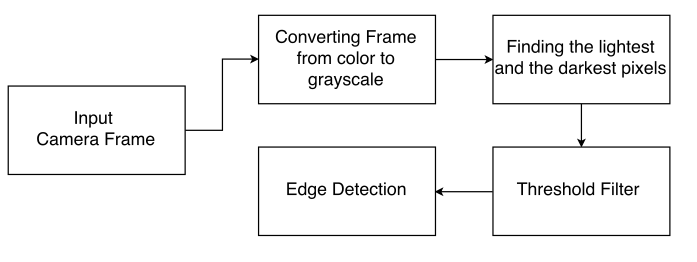
\includegraphics[width=1\textwidth]{./Bilder/Presprocessing_Figure.png}	
  \caption{Block Diagram of the Preprocessing Part}
  \label{fig:Block_Diagram_of_the_Preprocessing_Part}
\end{figure}





After the frame from Camera via ROS-Topic was received, the color frame had to be converted to a grayscale frame. For detection lanes, Hough Transformation is used and for Hough Transformation, the grayscale format of the input image is needed. Converting a frame from BGR format to grayscale format has some advantages, the main advantage being the processing time. Normally color frame matrix content has three or four channels, but grayscale frame matrix content has just one channel, so grayscale frame matrix size is much smaller compared to color frame matrix size. Because of this, the image processing time is much more less for the grayscale format compared to BGR format. In order to convert the BGR formatted frame to a grayscale formatted frame, the \textit{cvtColor} function from OpenCV is used.

For stable lane detection, the light conditions must be considered. Because of this, after converting the frame with BGR format to grayscale format, the lightest and darkest pixels have to be searched for. \emph{\color{blue}For the finding the lightest and the darkest pixels, the following function in OpenCV was used. This function will be explained in detail.}\cite{addWeighted}


\begin{center}

void minMaxLoc(InputArray src, double* minVal, double* maxVal=0, Point* minLoc=0, Point* maxLoc=0, InputArray mask=noArray())

\end{center}

\begin{itemize}

\item \textbf{src : }Input single channel array.

\item \textbf{minVal : }Pointer to the returned minimum value.

\item \textbf{maxVal : }Pointer to the returned maximum value.

\item \textbf{minLoc : }Pointer to the returned minimum location.

\item \textbf{maxLoc : }Pointer to the returned maximum location.

\item \textbf{mask : }Optional mask used to select a sub-array.

\end{itemize}


After finding the lightest and darkest pixels, it is possible to estimate the lighting conditions. These values are then used in the next step. After this processing, a filter is applied to all frames, transforming images into binary images by transforming each pixel according to whether it is inside or outside a specified range. The user chooses a threshold value to process. If a pixel is greater than this value, it is assigned an 'inside' value; otherwise, it is assigned an 'outside' value. Depending on the lightest and darkest pixel values, the threshold value changes. Through this dynamic parameter, the lanes are more able to be more clearly detected and noise can be cancelled more successfully. \emph{\color{blue}For this thresholding operation, the following function in OpenCV was used. This function will be explained in detail.}\citep{threshold}


\begin{center}

double threshold(InputArray src, OutputArray dst, double thresh, double maxval, int type)

\end{center}

\begin{itemize}

\item \textbf{src : }Input single channel array, which is 8-bit or 32-bit floating point.

\item \textbf{dst: }Output array which has the same size and type as src. 

\item \textbf{thresh : }Threshold value.

\item \textbf{maxval : }Maximum value to use with the THRESH\_BINARY and THRESH\_BINARY\_INV thresholding types.

\item \textbf{type : }Thresholding type, which can be THRESH\_BINARY, THRESH\_BINARY\_INV, THRESH\_TRUNC, THRESH\_TOZERO and THRESH\_TOZERO\_INV.

\end{itemize}






















After the threshold filter, an edge detection filter must be applied. In this master's thesis, the Sobel-Operator is used. This is explained in Chapter 2 in detail.
 
This preprocessing part is common for all cases but after this process, the cases diverge. 
 
%
\subsection{Method 1 : Hough Transformation + Rectangle Method + Curve Fitting + IPM}\label{sec:Case 1}

The algorithms and their orders which was used in this method, will be explained step by step. At Figure \ref{fig:Case1_BlockDiagram}, the block diagram of Method 1 is shown.



\begin{figure}[H]
 \centering
  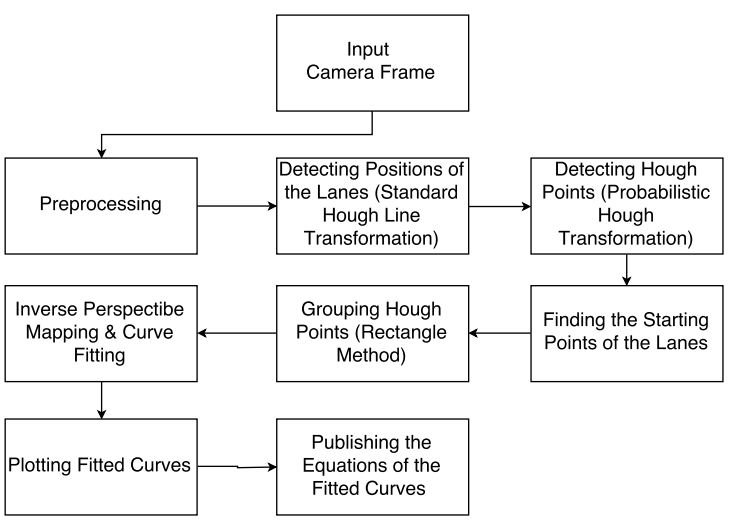
\includegraphics[width=1\textwidth]{./Bilder/Case1_BlockDiagram.png}		 \caption{Block Diagram of Case 1}
  \label{fig:Case1_BlockDiagram}
\end{figure}



\textbf{Step 1 : }As with all methods, the first step is preprocessing part. When the preprocessing part is over, the lanes must be detected. 

\textbf{Step 2 : }Secondly, the positions of the lanes should be found. In order to find the positions of the lanes, the Standard Hough Transformation is used. But the Standard Hough Transformation should not utilize the entire frame; rather, the frame is cropped. There is an advantage to cropping the frame, which will be explained in detail.


The frames obtained from the camera are at a resolution of 640x480 pixels, which is the default value. The resolution of the camera can be increased by adjusting its settings, but it is not possible to decrease it this way. In order to decrease the resolution of the camera, there is another technique that can be used. This technique is used with another method, and will be explained there. With this method, the minimum resolution the camera allows is used. There are some reasons for this, the most important being that if the resolution is increased, there are also more pixels, and thus the computing time increases as well. High computing time is of course undesirable.
 
The original height of the frame was 640 pixels, but as previously mentioned, the frame was cropped. As seen in Figure \ref{fig:Case1_withoutCropped}, when there is a curve, the camera also detects points that do not belong to the track. When the frame is not cropped, the detection of irrelevant points would result in the undesired production of red Standard Hough Transformation lines. As a result, first 100 pixels of the frame height were removed and the last 540 pixels were used. As seen at Figure \ref{fig:Case1_withCropped}, the red lines are shown only in the last 540 pixels of frame height and do not cover the irrelevant parts of the frame. If there is a lane, the red lines are very close each other, but if there is no lane, there is a distance of at least 50 pixels between the red lines. In Figure \ref{fig:Case1_withCropped}, there are three different groups of red lines. In each group, there is a lane. Thanks to the Standard Hough Line Transformation, we know which lanes are between which pixel columns.

\begin{figure}[H]
  \centering
  \subfloat[Hough Transformation without Cropping Image]{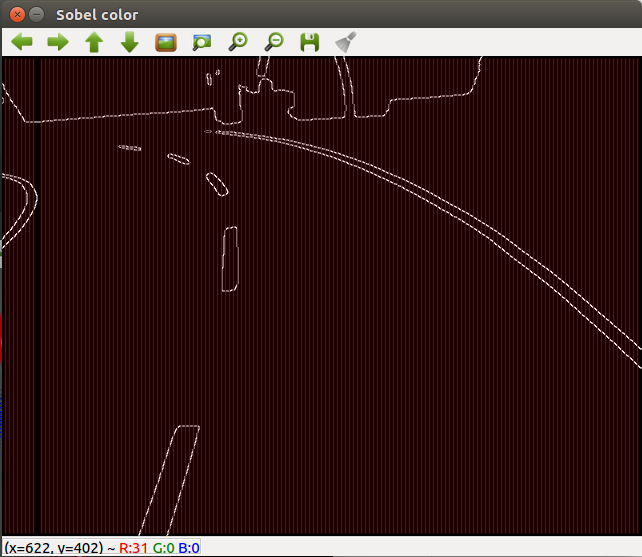
\includegraphics[width=0.45\textwidth]{./Bilder/Case1_withoutCropped.png}\label{fig:Case1_withoutCropped}}
  \hfill
  \subfloat[Hough Transformation with Cropping Image at Curve Lane]{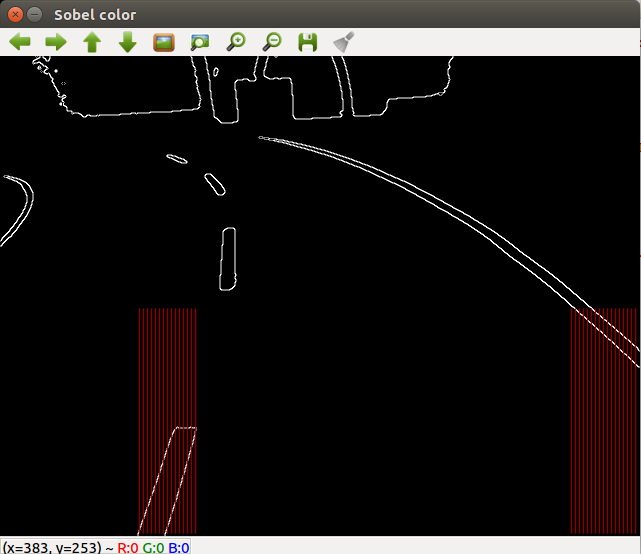
\includegraphics[width=0.45\textwidth]{./Bilder/Case1_withCropped.png}\label{fig:Case1_withCropped}}
  \caption{Detecting Lane Positions}
\end{figure}


But here there is also another problem. If a curve is to be detected, everything in this step works as it should (see Figure \ref{fig:Case1_withCropped}), but if a straight lane is to be detected, a problem occurs. As seen in Figure \ref{fig:Case1_Straight_Standard_Hough}, the beginning of the middle lane can be grouped with the left lane. In other words, there are again three different groups for three different lanes but each group of red lines fails to separate the lanes clearly from each other. As a result, the correct starting points of the middle and left lanes are not able to be found. In order for the lanes to be detected clearly, the frame must be divided into two horizontal rows.

As previously mentioned, 100 pixels were already cropped from the top of the image in order to detect the positions of the lanes clearly and now, the rest of the frame must be divided into two rows. Based on the experimental results, the top row is 150 pixels high and the bottom row is 230 pixels high. As a result, the lanes can be grouped into two small frames and in each small frame, the starting points of lanes must be found. As seen in Figure \ref{fig:Case1_Standard_Hough_Straight_2Parts}, when the frame is divided into two pieces, the lanes can be grouped separately.

\begin{figure}[H]
  \centering
  \subfloat[Hough Transformation with Cropping Image at Straight Lane in 1 piece]{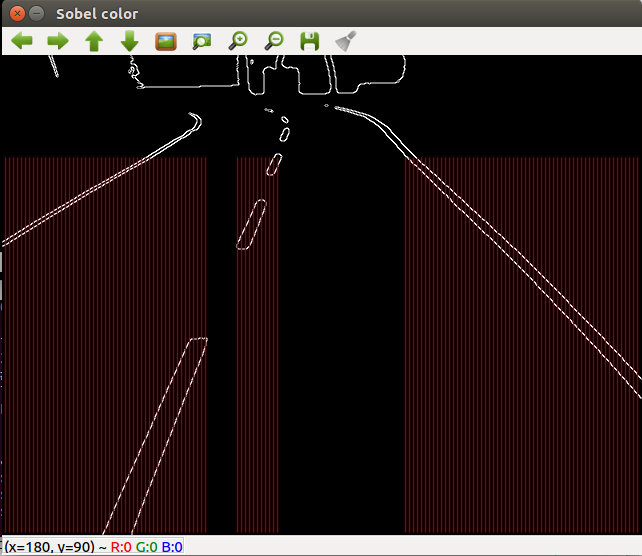
\includegraphics[width=0.45\textwidth]{./Bilder/Case1_Straight_Standard_Hough.png}\label{fig:Case1_Straight_Standard_Hough}}
  \hfill
  \subfloat[Hough Transformation with Cropping Image at Straight Lane in 2 pieces]{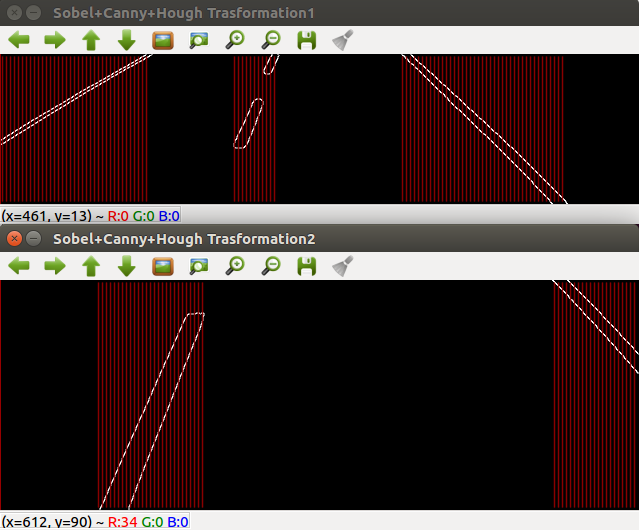
\includegraphics[width=0.45\textwidth]{./Bilder/Case1_Standard_Hough_Straight_2Parts.png}\label{fig:Case1_Standard_Hough_Straight_2Parts}}
  \caption{Standard Hough Transformation in Straight Lanes}
\end{figure} 


\textbf{Step 3 : }After the lanes are grouped separately in two different small frames, the heights of which are 230 and 150 pixels, the points (pixels) on the lanes must be found in two small frames. For that, we have to use Probabilistic Hough Transformation. The Probabilistic Hough Transformation is a bit different than Standard Hough Line Transformation because Standard Hough Transformation is more suitable for straight lanes. However, if there is a curve, the Standard Hough Transformation is not able to detect lanes very well. As previously mentioned, a line can be represented as y = mx+c or in parametric form, as $\rho$ = x $\cos \theta$ + y$ \sin \theta$ where  $\rho$ is the perpendicular distance from origin to the line, and $\theta$ is the angle formed by this perpendicular line and horizontal axis measured in counter-clockwise. However, is different in the case of the Probabilistic Hough Transformation. A line is represented by two or more points. If the Probabilistic Hough Transformation finds at least two points from the same line, it represents the two end points of these lines.

In this master's thesis, the Probabilistic Hough lines are not drawn because just the points (pixels) which are detected in the lanes with the Probabilistic Hough Transformation are needed. 


\begin{figure}[H]
  \centering
  \subfloat[Original Image with Probabilistic Hough Transformation]{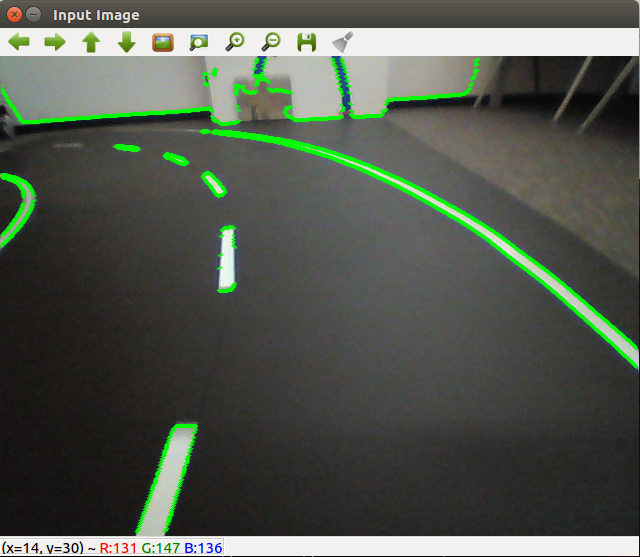
\includegraphics[width=0.45\textwidth]{./Bilder/Case1_HoughPoints_Original.png}\label{fig:Case1_HoughPoints_Original}}
  \hfill
  \subfloat[A Image with Sobel Operator and Probabilistic Hough Transformation]{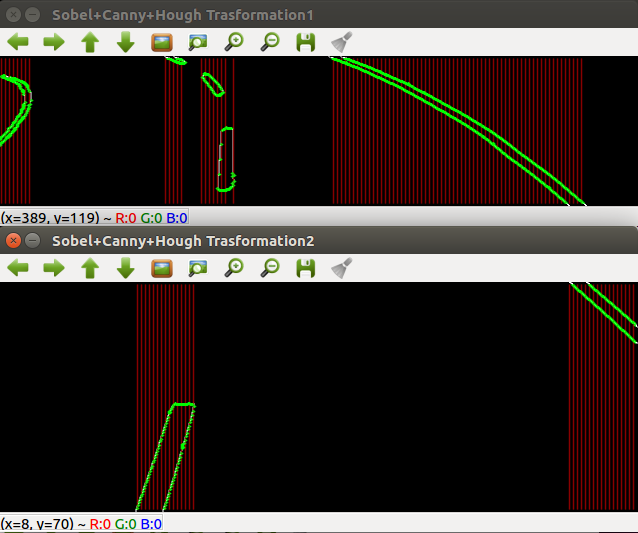
\includegraphics[width=0.45\textwidth]{./Bilder/Case1_HoughPoints_Sobel.png}\label{fig:Case1_HoughPoints_Sobel}}
  \caption{Probabilistic Hough Transformation Points}
\end{figure} 
 
In Figure \ref{fig:Case1_HoughPoints_Original} and Figure \ref{fig:Case1_HoughPoints_Sobel}, the Probabilistic Hough Transformation Points (green pixels) are shown. The Probabilistic Hough Transformation detected a large number of pixels. By changing the parameters of the Probabilistic Hough Transformation found in OpenCV, fewer Hough Points on the lanes are able to be detected, but detecting too few Hough points can also cause some problems for detecting the lanes. On the other hand, detecting a large number of Hough Points results in more computing time, which is undesirable. So in this case, the parameters of Probabilistic Hough Transformation fuction in OpenCV must be optimized. Thanks to optimization, the best solution (less computing time and good lane detection) is found.

\textbf{Step 4 : }It is now known in which pixel columns the lanes lie (Step 2), and the points (pixels) on the lanes are also shown thanks to the Probabilistic Hough Transformation (Step 3), and after these two steps, the starting points (pixels) of the lanes can be found. In order to do that, the Hough Points for each group of Hough lines that were found in Step 2 are compared with each other, and then the last pixels in the columns should be found. If the camera can see three lanes, then the different starting points for the three different lanes must be found. This means that this process must be done for all lanes which can be seen in the frame.


\textbf{Step 5 : }The next step in this method is getting the Hough Points which are relevant to the lanes. Now, for each lane, the Hough Points must be also grouped. For getting the Hough Points which are relevant to the lanes, what I term the 'rectangle' method is to be used. In the rectangle method, a rectangle is drawn for each lane at the starting point found in Step 4, and the coordinates of all of the Hough Points in that rectangle are saved in a vector. The highest Hough Point in the rectangle must then be found. From that point, another rectangle must be drawn, but the sizes of the rectangles are becoming progressively smaller, because the objects seem smaller the further away they are from the camera. The sizes of the rectangles are also similar but there is an exception with regard to the middle lane. The middle lane has dashed lines so the rectangles in the middle lane must be bigger than in the left and right lanes. As seen in Figure \ref{fig:Case1_Rectangles} (rectangles shown in blue), with this method, the noise and the Hough Points which are not relevant to the lanes are removed.


\begin{figure}[H]
 \centering
  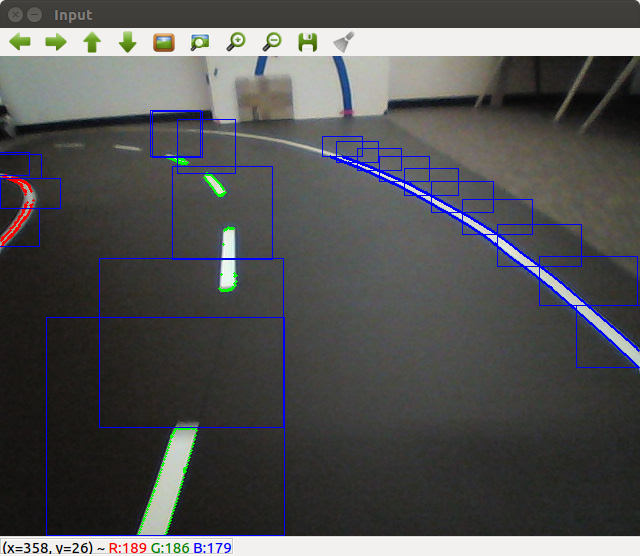
\includegraphics[width=0.45\textwidth]{./Bilder/Case1_Rectangles.png}\label{fig:Case1_Rectangles}
	\caption{Rectangle Method}
\end{figure}


\textbf{Step 6 : }The next step of this method is curve fitting. Curve Fitting is an algorithm which gives a mathematical description and this mathematical description provides the best fit for a series of data points. But in this master's thesis, the curve fitting to be performed is modified. In this curve fitting, the coordinates of Hough Points are used but the x and y coordinates of these Hough Points are swapped, because the y-axes of these coordinates have more range than the x-axes. As a result, this swap raises the stability of the curve fitting.

After using the Hough Points as input, three different mathematical equations are produced. One of these equations is for the left lane, another is for the middle lane, and the last equation is for the right lane. In order to produce these equations, naturally, only the relevant Hough points are used. For example, for left lane curve equation, only the Hough Points from the left lane were used.
 
\textbf{Step 7 : }The next step of this method is plotting the fitted curves produced by the curve fitting function. We start from first pixel and continue to the 480th pixel vertically and the output values of the equation for each pixel in the column are found. For each lane, the fitted curves are plotted in different color. In Figure \ref{fig:Case1_CurveFittingwithoutIPM.png}, the fitted curve can be seen.


\begin{figure}[H]
 \centering
  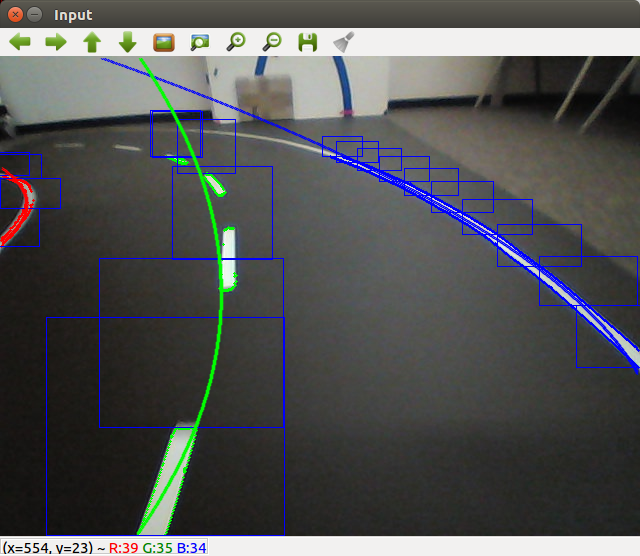
\includegraphics[width=0.45\textwidth]{./Bilder/Case1_CurveFittingwithoutIPM.png}\label{fig:Case1_CurveFittingwithoutIPM.png}
	\caption{Fitted Curve}
\end{figure}


 
\textbf{Step 8 : }Until this step, the fitted curves were plotted from the camera view, but at the end of the project, the fitted curves of the lanes need to be able to be seen from a bird's-eye view. As a result, the perspective of lanes must be changed from the camera side to the top of the track side. This step can be termed 'Inverse Perspective Mapping(IPM)'. For IPM, a function from OpenCV, which is called 'findHomography', was used. Thanks this function, all fitted curve points can be converted to the perspective of the top of the track side. It was also possible to convert all pixels from the camera perspective to the top of the track perspective, but in that case, it would have been necessary to convert 640x480 pixels, which means 307200 pixels in total. In this case, it is only necessary to convert 480 pixels for each lane, and so 1440 pixels in total. As a result, this method is more efficient than converting all pixels.
 	 		 	
\begin{figure}[H]
  \centering
  \subfloat{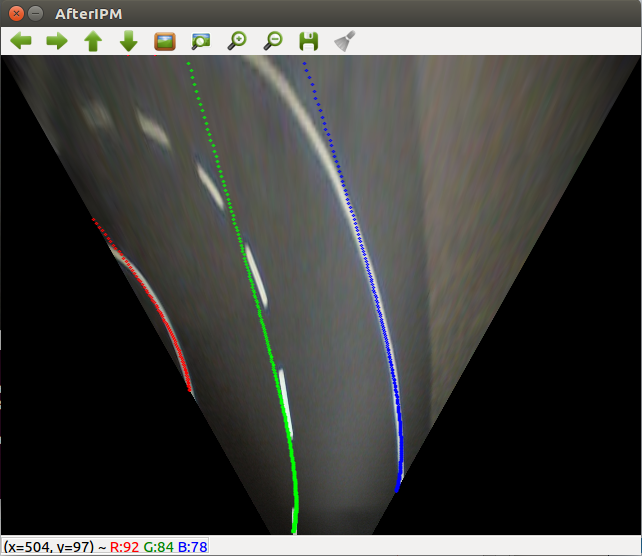
\includegraphics[width=0.45\textwidth]{./Bilder/Case1_CurveFitting.png}\label{fig:Case1_CurveFitting}}
  \caption{Curve Fitting}
\end{figure} 


\textbf{Step 9 : }The last step of this method is publishing the coefficients of the equations of the fitted curves from the bird's-eye view. In order to activate the automobile for autonomous driving, only the equations of the fitted curves are needed. For this step, a ROS Topic must be created. The frequency of the rostopics can be adjusted.

%

\subsection{Method 2 : IPM + Hough Transformation + KNN + Curve Fitting}\label{sec:Case 2}

\begin{figure}[H]
 \centering
  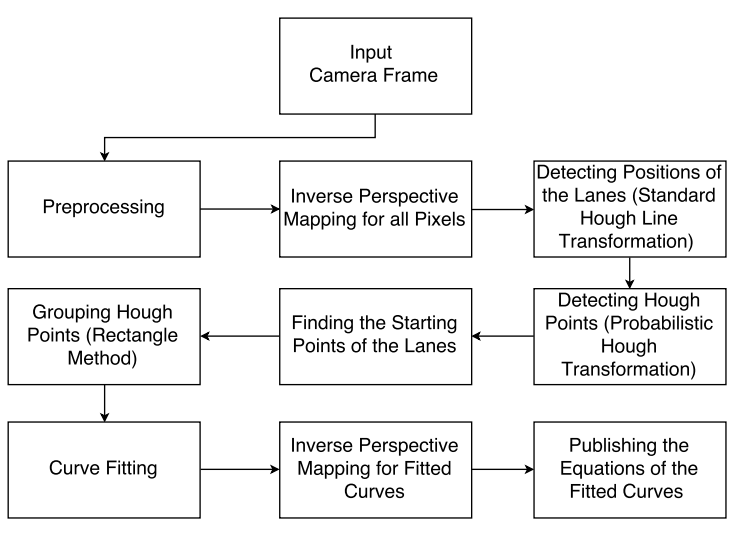
\includegraphics[width=1\textwidth]{./Bilder/Case2_BlockDiagram.png}\label{fig:Case2_BlockDiagram}
	\caption{Block Diagram of Case 2}
\end{figure}

\textbf{Step 1 : }As previously mentioned, the preprocessing part is common for all methods. So in this method, the preprocessing part was also the first step.

\textbf{Step 2 : }In this method, the frames taken from the camera, are converted directly from the camera perspective to the bird's-eye view perspective. In Section \ref{sec:Case 1} (Method 1), only the curve fitting pixels were converted from the camera perspective to the top of the truck perspective. The time needed to convert 640x480 pixels (307200 pixels in total) is a bit more when compared to Method 1. The original frame, which can be seen in Figure \ref{fig:Case2_InputImg}, is converted to the frame which can be seen in Figure \ref{fig:Case2_IPM} by OpenCV 'findHomography' function.

 
\begin{figure}[H]
  \centering
  \subfloat[Original Image]{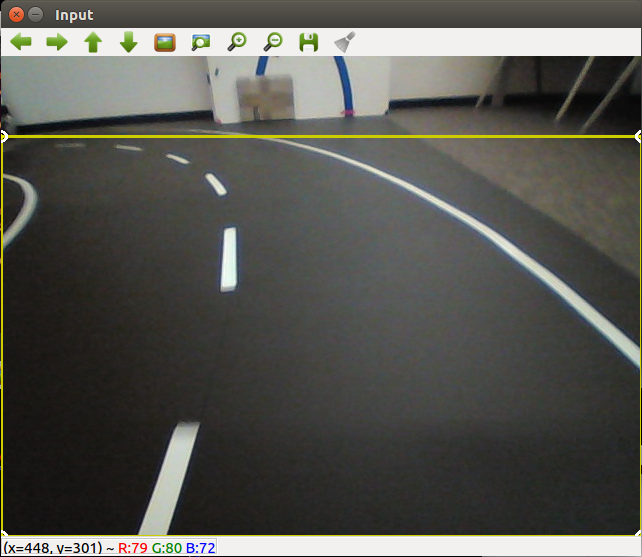
\includegraphics[width=0.45\textwidth]{./Bilder/Case2_InputImg.png}\label{fig:Case2_InputImg}}
  \hfill
  \subfloat[A Image with Inverse Perspective Mapping]{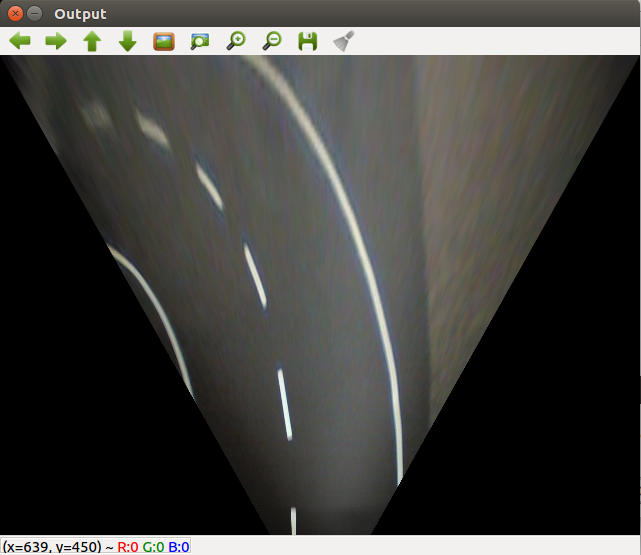
\includegraphics[width=0.45\textwidth]{./Bilder/Case2_IPM.png}\label{fig:Case2_IPM}}
  \caption{Inverse Perspective Mapping}
\end{figure} 


\textbf{Step 3 : }The next step of this method is finding the vertical pixels which the lanes lie between. In Method 1(Section \ref{sec:Case 1}, the first 100 pixels from the top of the frame were cropped and then rest of the frame was divided into two pieces. This was necessary because otherwise, the straight lanes would have caused a problem in the grouping of the lanes. In this method, it is not necessary to crop the frame. In Method 1, except for the first 100 pixels of the frame, it was necessary to apply the Standard Hough Line Transformation for 380x640 pixels. In this methood, it sufficient to apply the Standard Hough Line Transformation to only the last 200 pixels of the frame, because these 200 pixels are able to cover all lanes in the frame. In Figure \ref{fig:Case2_Standard_Hough_Transformation}, all lanes can be distinguished thanks to the Hough lines. 


\begin{figure}[H]
  \centering
  \subfloat{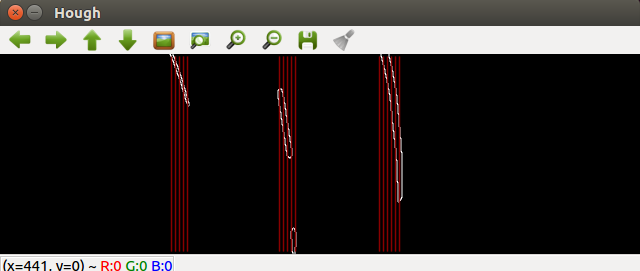
\includegraphics[width=0.45\textwidth]{./Bilder/Case2_Standard_Hough_Transformation.png}\label{fig:Case2_Standard_Hough_Transformation}}
  \caption{Standard Hough Line Transformation after IPM Method}
\end{figure} 



\textbf{Step 4 : }After finding which pixel columns the lanes lie between in Step 3, the Probabilistic Hough Transformation was used. Thanks to Probabilistic Hough Transformation, the Hough Points appear on the lanes. As mentioned in Method 1 in Section \ref{sec:Case 1}, there are some parameters in Probabilistic Hough Transformations, so the number of Hough Points can be descreased or increased. Decreasing the number of Hough Points also decreases the computing time but decreasing the number of Hough Points by too much can decrease the accuracy of lane detection. Therefore, the parameters must be set in an optimal way.

\textbf{Step 5 : }We have already found out which pixel columns the lanes lie between. The Hough Points must now be grouped according to lanes. If the camera can see all three lanes, then there must also be three different groups of Hough Points. However, if there is a curve, the camera can see just the right and middle lane, so the Hough Points must be grouped into two groups in this case. For each lane, the starting points of the lanes must be found. For that, all Hough Points in a group must be compared with each other. The Hough Points which are the closest to the bottom of the frame are the starting points.

\textbf{Step 6 : }The next step of this method is the k-nearest neighbors algorithm (KNN). KNN is a learning algorithm. Here KNN is used instead of the rectangle method used in Method 1. The KNN algorithm divides the frames into some equal-sized pieces. The nearest neighbor points are found in each piece. This process begins from the starting points of the lanes which were found in Step 5. The KNN functions are used from OpenCV. There are some parameters in these functions. For example, we can set the number of neighbor points to be found. The parameters must be set optimally, meaning the project must work fast and efficiently.

\textbf{Step 7 : }After finding the points from KNN in Step 6, which are to be used as the input values of the curve fitting function, then the function of the curve fitting is applied. The advantage of the KNN algorithm is that it does not return so many Hough Points, which are the input values of the curve fitting, when compared to rectangle method. So here, the curve fitting function produces the mathematical equations of the lane much faster when compared to Method 1.

\textbf{Step 8 : }After the equations of the fitted curves for each of the lanes are calculated, these equations have to be plotted like in Method 1. Here, the x and y coordinates of the Hough Points were also swapped in order to get more stable curves. For each of the vertical pixels, the results of all of the equations were plotted in the frame.


\textbf{Step 9 : }The last step of this method is also to publish the coefficients of the equations of the fitted curves of each of the lanes which can be seen by the camera.


\begin{figure}[H]
  \centering
  \subfloat{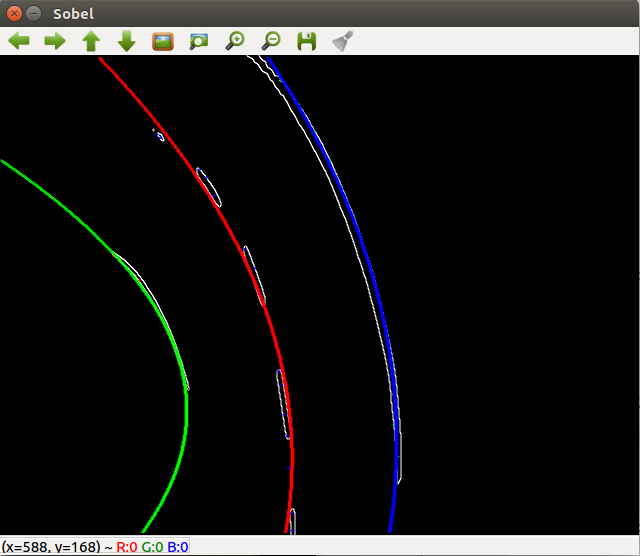
\includegraphics[width=0.45\textwidth]{./Bilder/Case2_OutputImage.png}\label{fig:Case2_OutputImage}}
  \caption{Output Image}
\end{figure} 


\subsection{Method 3 : IPM + Hough Transformation + Rectangle Method + Curve Fitting}\label{sec:Case 3}

This method is a composite method of the Method 1 in Section \ref{sec:Case 1} and Method 2 in Section \ref{sec:Case 2}. As in Method 2, at the beginning of this method, the preprocessing part is applied, and then Inverse Perspective Mapping for all pixels is implemented. After that, for 200x640 pixels, the Standard Hough Transformation is used and then for all pixels Probabilistic Hough Transformation is implemented. Until this point, the implementation is completely identical to Method 2. In Method 2, however, at the point in the process where the k-nearest neighbours (KNN) method is used, the rectangle method used in Method 1 in Section \ref{sec:Case 1} is applied. There is, however, a difference between the rectangle method utilized here and the rectangle method from Method 1. In Method 1, the size of rectangles decreased progressively. However, in this method, the size of the rectangles is always the same because the Inverse Perspective Method(IPM) is used at the beginning. As a result, the lanes are shown from the top of track. The size of the rectangles in the middle lane is bigger than the size of the rectangles in the left and right lanes, however. Because of the dashed lines, it was necessary to use larger rectangles in the middle lane.

After the rectangle method is used, the curve fitting method is used. As with the other methods, the x and y coordinates of Probabilistic Hough Points are swapped after the rectangle method is applied. Thanks to this swap, the curve fitting is more accurate. After producing three different equations for three different lanes, the output values for all pixel columns are calculated and plotted in the frame. In Figure \ref{fig:Case3_OutputImage}, the fitted curves are shown.

The last step of this method is as in the others: to publish the equations of the fitted curves produced from the lanes. These fitted curves are published with Ros Topics.

\begin{figure}[H]
  \centering
  \subfloat{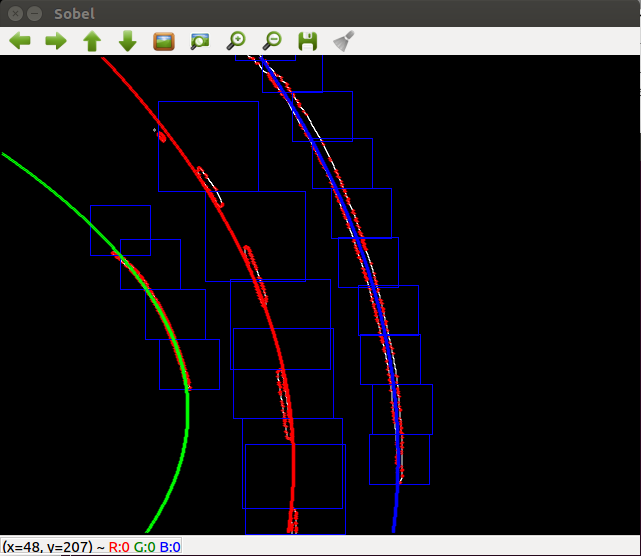
\includegraphics[width=0.45\textwidth]{./Bilder/Case3_OutputImage.png}\label{fig:Case3_OutputImage}}
  \caption{Output Image}
\end{figure}

\subsection{Method 4 : Resize + IPM + Hough Transformation + KNN + Curve Fitting}\label{sec:Case 4}

This method is very similar to Method 2. There is just one difference between Method 2 in \ref{sec:Case 2} and this method. The only difference is resizing the frame at the beginning. The frame comes from the camera with a 640x480 pixel resolution, but this frame is resized from a 640x480 pixel resolution to a 320x240 pixel resolution. In order to do this, a 'resize' function from OpenCV is used because the smallest resolution able to be obtained from the camera is 640x480 pixels. Due to the resizing, it was sometimes necessary to use different parameters than in Method 2 in order to detect lanes optimally (efficiently and accurately). Results of this method are shown in Figure \ref{fig:Case4_OutputImage}.

\begin{figure}[H]
  \centering
  \subfloat{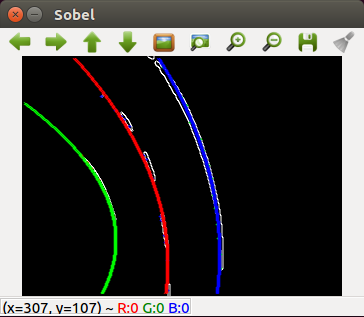
\includegraphics[width=0.45\textwidth]{./Bilder/Case4_OutputImage.png}\label{fig:Case4_OutputImage}}
  \caption{Output Image(320x240 pixels resolution)}
\end{figure}





\subsection{Method 5 : Resize + Hough Transformation + Rectangle Method + Curve Fitting + IPM}\label{sec:Case 5}
%
